\documentclass[tikz,border=4pt]{standalone}
\usepackage{xcolor}
\usetikzlibrary{arrows.meta,positioning,calc}

\newcommand{\pyfun}[1]{{\ttfamily\textcolor{blue!65!black}{def} \textcolor{black}{#1}\textcolor{black}{():}}}

\begin{document}
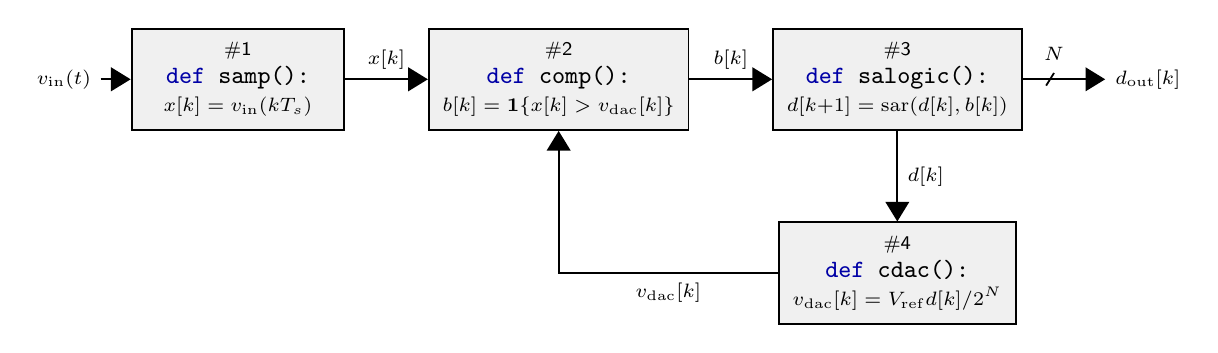
\begin{tikzpicture}[
  font=\sffamily\small,
  block/.style={draw=black, line width=0.7pt, fill=black!6, rectangle, minimum width=2.7cm, minimum height=1.18cm, align=center, inner sep=5pt},
  arr/.style={-{Triangle[length=2.5mm,width=3.0mm]}, line width=0.75pt, draw=black},
  sig/.style={font=\ttfamily\scriptsize, text=black},
  expr/.style={font=\sffamily\scriptsize, text=black},
]
  \node[block] (samp) at (0,0) {{\scriptsize \#1}\\[-1pt]\pyfun{samp}\\[-1pt]{\scriptsize $x[k]=v_{\mathrm{in}}(kT_s)$}};
  \node[block, right=1.05cm of samp] (comp) {{\scriptsize \#2}\\[-1pt]\pyfun{comp}\\[-1pt]{\scriptsize $b[k]=\mathbf{1}\{x[k]>v_{\mathrm{dac}}[k]\}$}};
  \node[block, right=1.05cm of comp] (logic) {{\scriptsize \#3}\\[-1pt]\pyfun{salogic}\\[-1pt]{\scriptsize $d[k{+}1]=\mathrm{sar}(d[k],b[k])$}};
  \node[block, below=1.15cm of logic] (dac) {{\scriptsize \#4}\\[-1pt]\pyfun{cdac}\\[-1pt]{\scriptsize $v_{\mathrm{dac}}[k]=V_{\mathrm{ref}}d[k]/2^N$}};

  \node[sig, left=0.38cm of samp] (vin) {$v_{\mathrm{in}}(t)$};
  \draw[arr] (vin) -- (samp.west);
  \draw[arr] (samp.east) -- node[sig, above] {$x[k]$} (comp.west);
  \draw[arr] (comp.east) -- node[sig, above] {$b[k]$} (logic.west);
  \coordinate (dout) at ($(logic.east)+(1.05,0)$);
  \draw[arr] (logic.east) -- (dout) node[font=\scriptsize, right] {$d_{\mathrm{out}}[k]$};
  \draw[line width=0.65pt, draw=black] ($(logic.east)+(0.30,-0.08)$) -- ($(logic.east)+(0.40,0.08)$) node[font=\scriptsize, above=1pt] {$N$};
  \draw[arr] (logic.south) -- node[sig, right] {$d[k]$} (dac.north);
  \draw[arr] (dac.west) -| node[pos=0.25, below, sig] {$v_{\mathrm{dac}}[k]$} ($(comp.south)+(0,-0.35)$) -- (comp.south);
\end{tikzpicture}
\end{document}
